\documentclass[12pt,letterpaper]{ctexart}
\usepackage{fullpage}
\usepackage[top=2cm, bottom=4.5cm, left=2.5cm, right=2.5cm]{geometry}
\usepackage{amsmath,amsthm,amsfonts,amssymb,amscd}
\usepackage{lastpage}
\usepackage{enumerate}
\usepackage[binary-units=true]{siunitx}
\usepackage{fancyhdr}
\usepackage{mathrsfs}
\usepackage{xcolor}
\usepackage{graphicx} %插入图片的宏包
\usepackage{float} %设置图片浮动位置的宏包
\usepackage{subfigure} %插入多图时用子图显示的宏包
\usepackage{listings}
\usepackage{afterpage}
\usepackage{hyperref}
\hypersetup{
    colorlinks=true,
    linkcolor=blue,
    filecolor=magenta,
    urlcolor=cyan,
}

\newcommand\blankpage{%
  \null
  \thispagestyle{empty}%
  \addtocounter{page}{-1}%
  \newpage
}


\hypersetup{%
  colorlinks=true,
  linkcolor=blue,
  linkbordercolor={0 0 1}
}

\renewcommand\lstlistingname{Algorithm}
\renewcommand\lstlistlistingname{Algorithms}
\def\lstlistingautorefname{Alg.}

\lstdefinestyle{Python}{
    language        = Python,
    frame           = lines,
    basicstyle      = \footnotesize,
    keywordstyle    = \color{blue},
    stringstyle     = \color{green},
    commentstyle    = \color{red}\ttfamily
}

\setlength{\parindent}{0.0in}
\setlength{\parskip}{0.05in}

% Edit these as appropriate
\newcommand\course{CS305}
\newcommand\hwnumber{10}                  % <-- homework number
\newcommand\NetIDa{11711918}              % <-- NetID of person #1
\newcommand\NetIDb{吴烨昌}                 % <-- NetID of person #2 (Comment this line out for problem sets)

\pagestyle{fancyplain}
\headheight 35pt
\lhead{\NetIDa}
\lhead{\NetIDa\\\NetIDb}                 % <-- Comment this line out for problem sets (make sure you are person #1)
\chead{\textbf{\Large Assignment \hwnumber}}
\rhead{\course \\ \today}
\lfoot{}
\cfoot{}
\rfoot{\small\thepage}
\headsep 1.5em

\begin{document}

\section*{Problem 1}

{\bf Description}

Initiates an ICMP session to test if www.example.com is reachable(setting the packet size is 3200B ), capture the packets.
\begin{enumerate}
  \item How to initiates an ICMP Echo request with 3200B length?
  \item Is there any fragmentation on the IP packets , how do you find it?
  \item How many fragments of a 3200B length IP packet?
  \item How do you identify the ICMP Echo request and Echo reply?
  \item For the ICMP Echo request, which fragment is the 1st one, which is the last? How do you identify them?
  \item What’s the length of each IP fragment? Is the sum of each fragment’s length equal to the original IP packet?
\end{enumerate}


{\bf Solution}


\begin{enumerate}
  \item Use \verb|ping -4 www.example.com -l 3200|.
  \item Use \verb|icmp && !(ip.flags.mf eq 0)| to filter all ICMP packet with that MF flag is not 0(which means it has more fragments).
  \begin{figure}[H]
    \centering
    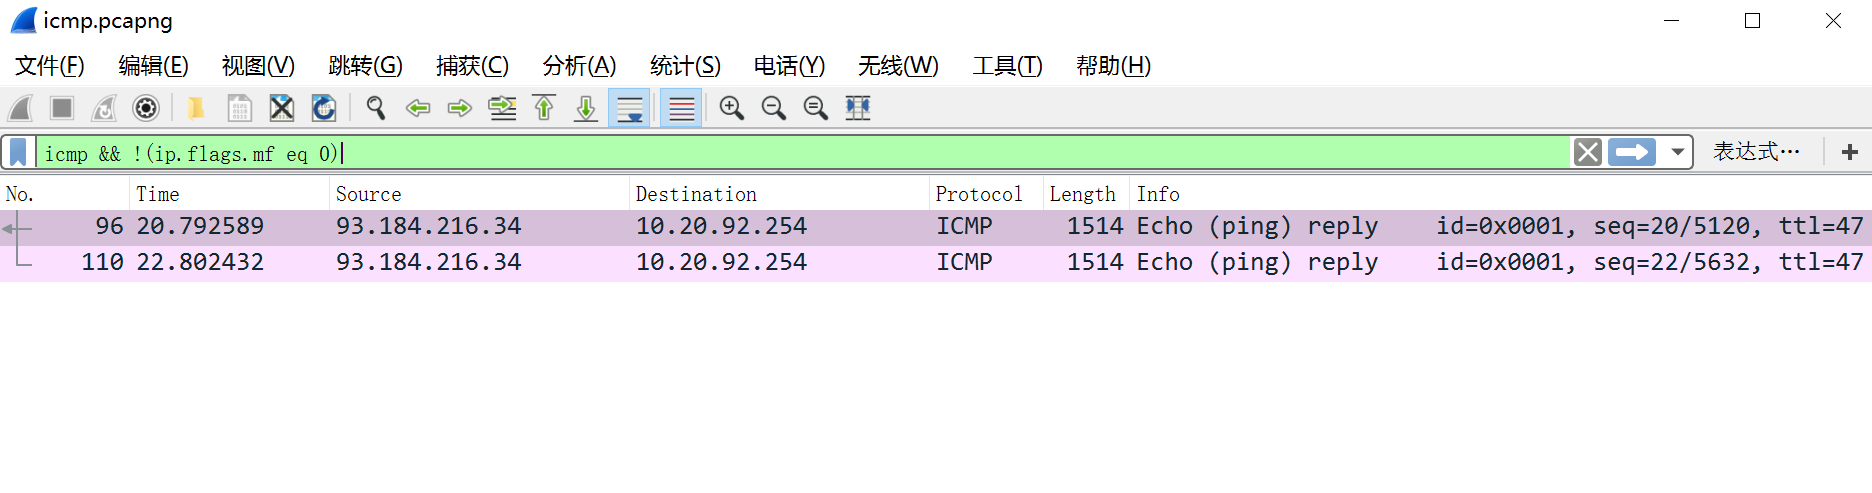
\includegraphics[width=0.8\linewidth]{assets/icmp_mf.png}
    \caption{ICMP packet with fragment}
  \end{figure}
  \item Use \verb|ip.id == 51941|, 3 fragment can be found.
  \begin{figure}[H]
    \centering
    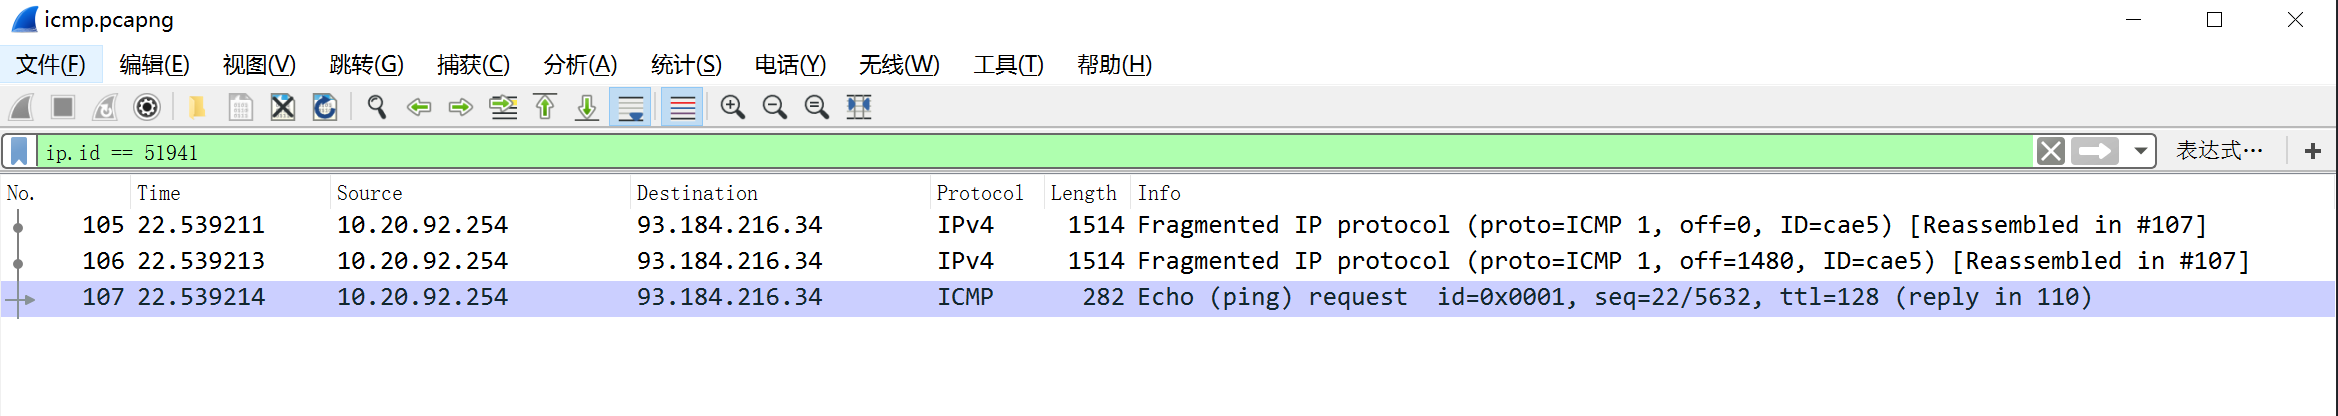
\includegraphics[width=0.8\linewidth]{assets/ip_fragment.png}
    \caption{ICMP packet with fragment}
    \label{fig:packet_with_fragment}
  \end{figure}
  \item By checking the type of ICMP packet. 8 stands for request and 0 stands for reply.
  \item From Figure~\ref{fig:packet_with_fragment}, \#105 is the first fragment and \#107 is the last fragment. It can be identified by offset field.
  The offset of fragments is increasing so the first fragment has 0 as its offset and the last fragment has a maximum offset.
  \item The length of first two fragments are 1500, the length of the third one is 268.
  I apply length as column. The first two fragments has 1480B data and 20B IP header. The third one has 280B data, 8B ICMP header and 20B IP header.
  The sum of each fragment's length is $1500 + 1500 + 268 = 3268$, the original IP packet's length should be $20 + 8 + 3200 = 3228$.
  They are not the same.
  \begin{figure}[H]
    \centering
    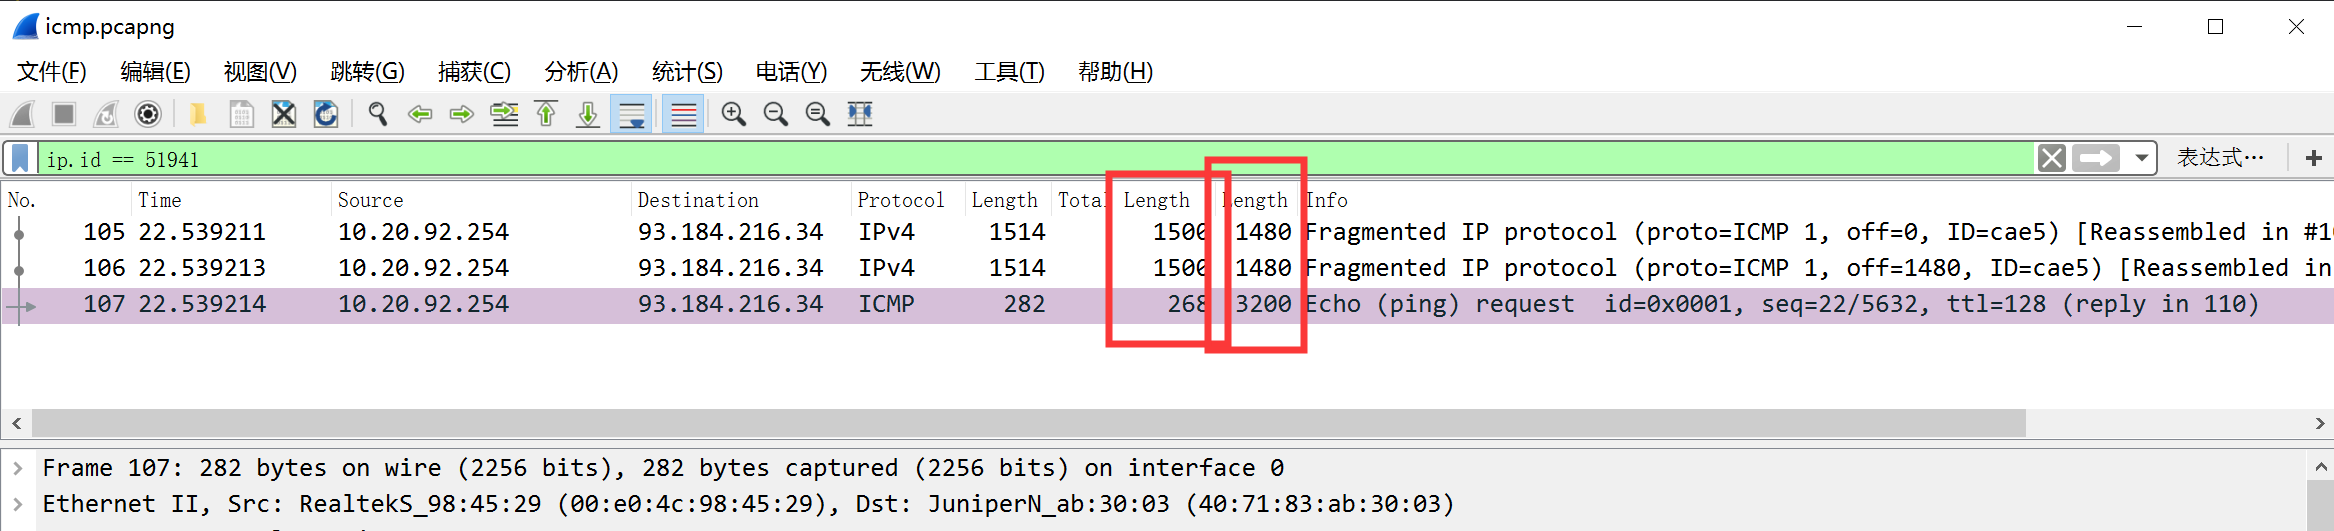
\includegraphics[width=0.8\linewidth]{assets/ip_length.png}
    \caption{ICMP packet with length}
    \label{fig:packet_with_length}
  \end{figure}
\end{enumerate}

\newpage

\section*{Problem 2}

{\bf Description}

Using tracert (windows) / traceroute(linux or MacOS) to trace the route from your host to www.sustech.edu.cn. Capture the packets while tracing.

\begin{enumerate}
  \item Is there any ‘Time-to-live exceeded’ ICMP packets?
  \item What’s the difference between these packets and normal ICMP packets(such as ICMP echo request)? List at least 3 aspects.
\end{enumerate}

Please add the necessary screenshots when answering questions



{\bf Solution}


\begin{enumerate}
  \item Yes, there are.
  \begin{figure}[H]
    \centering
    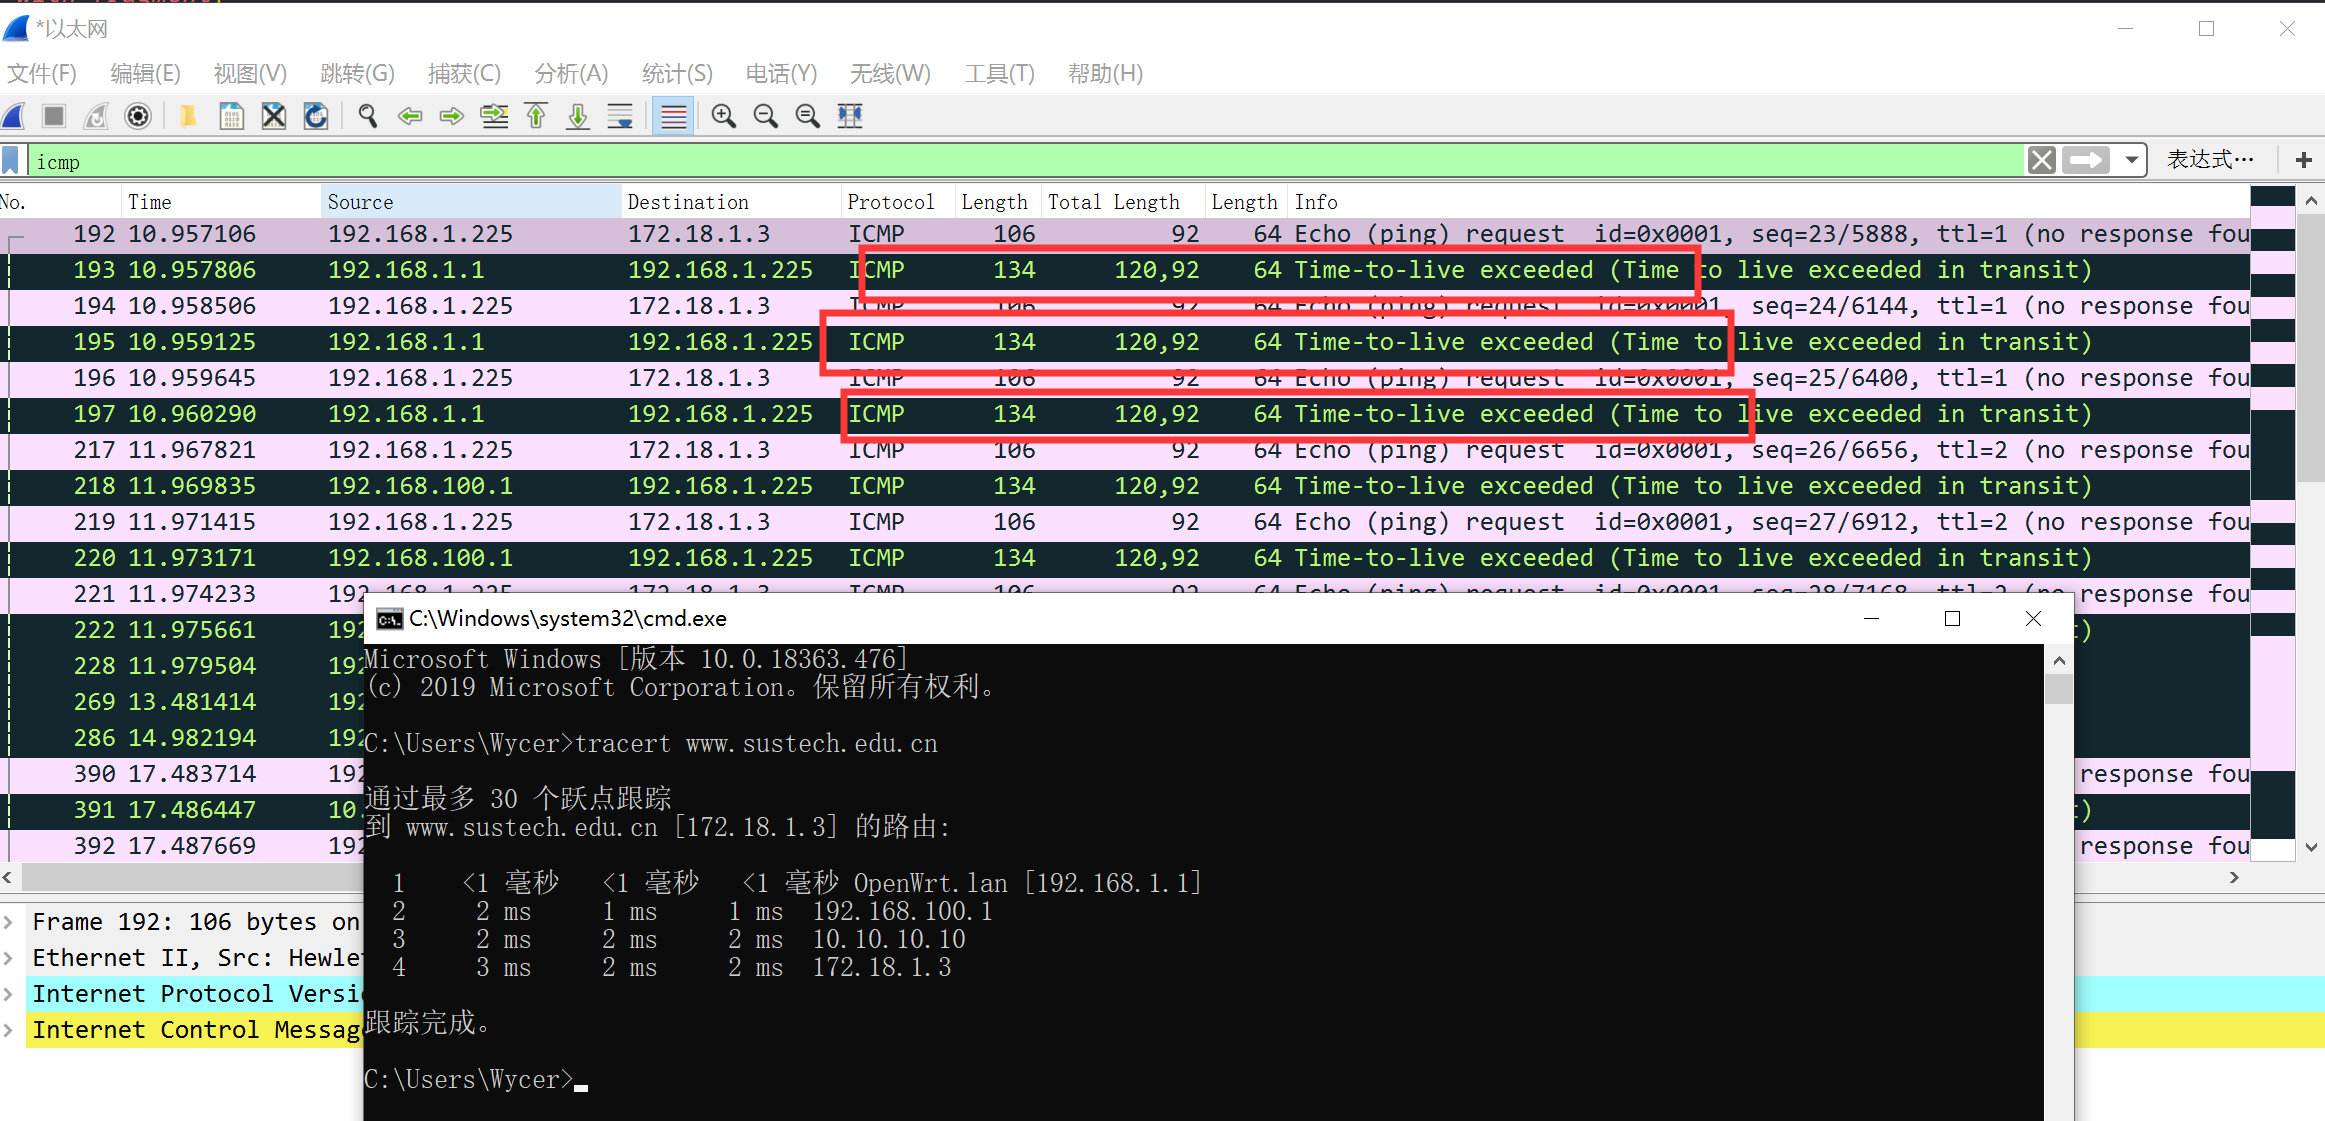
\includegraphics[width=0.8\linewidth]{assets/TTL.png}
    \caption{TTL exceeded packets when tracert}
    \label{fig:packet_with_length}
  \end{figure}
  \item As follows
  \begin{enumerate}
    \item They has different types.
    \begin{figure}[H]
      \centering
      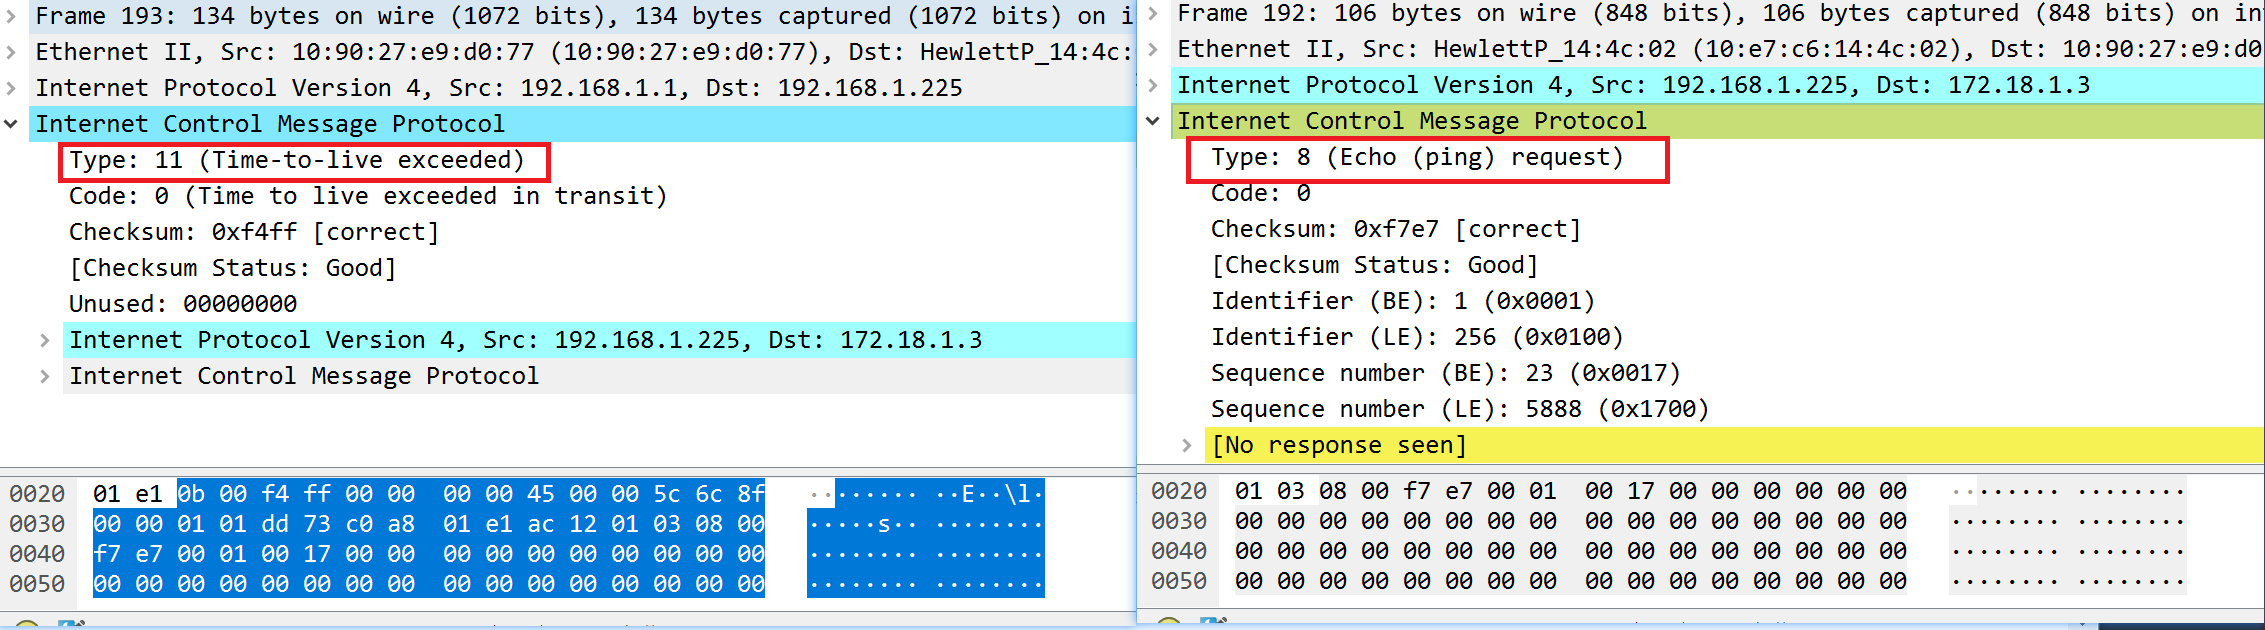
\includegraphics[width=0.8\linewidth]{assets/diff1.png}
      \caption{Different types}
    \end{figure}
    \item The TTL-exceeded packet has a IPv4 datagram in it.
    \begin{figure}[H]
      \centering
      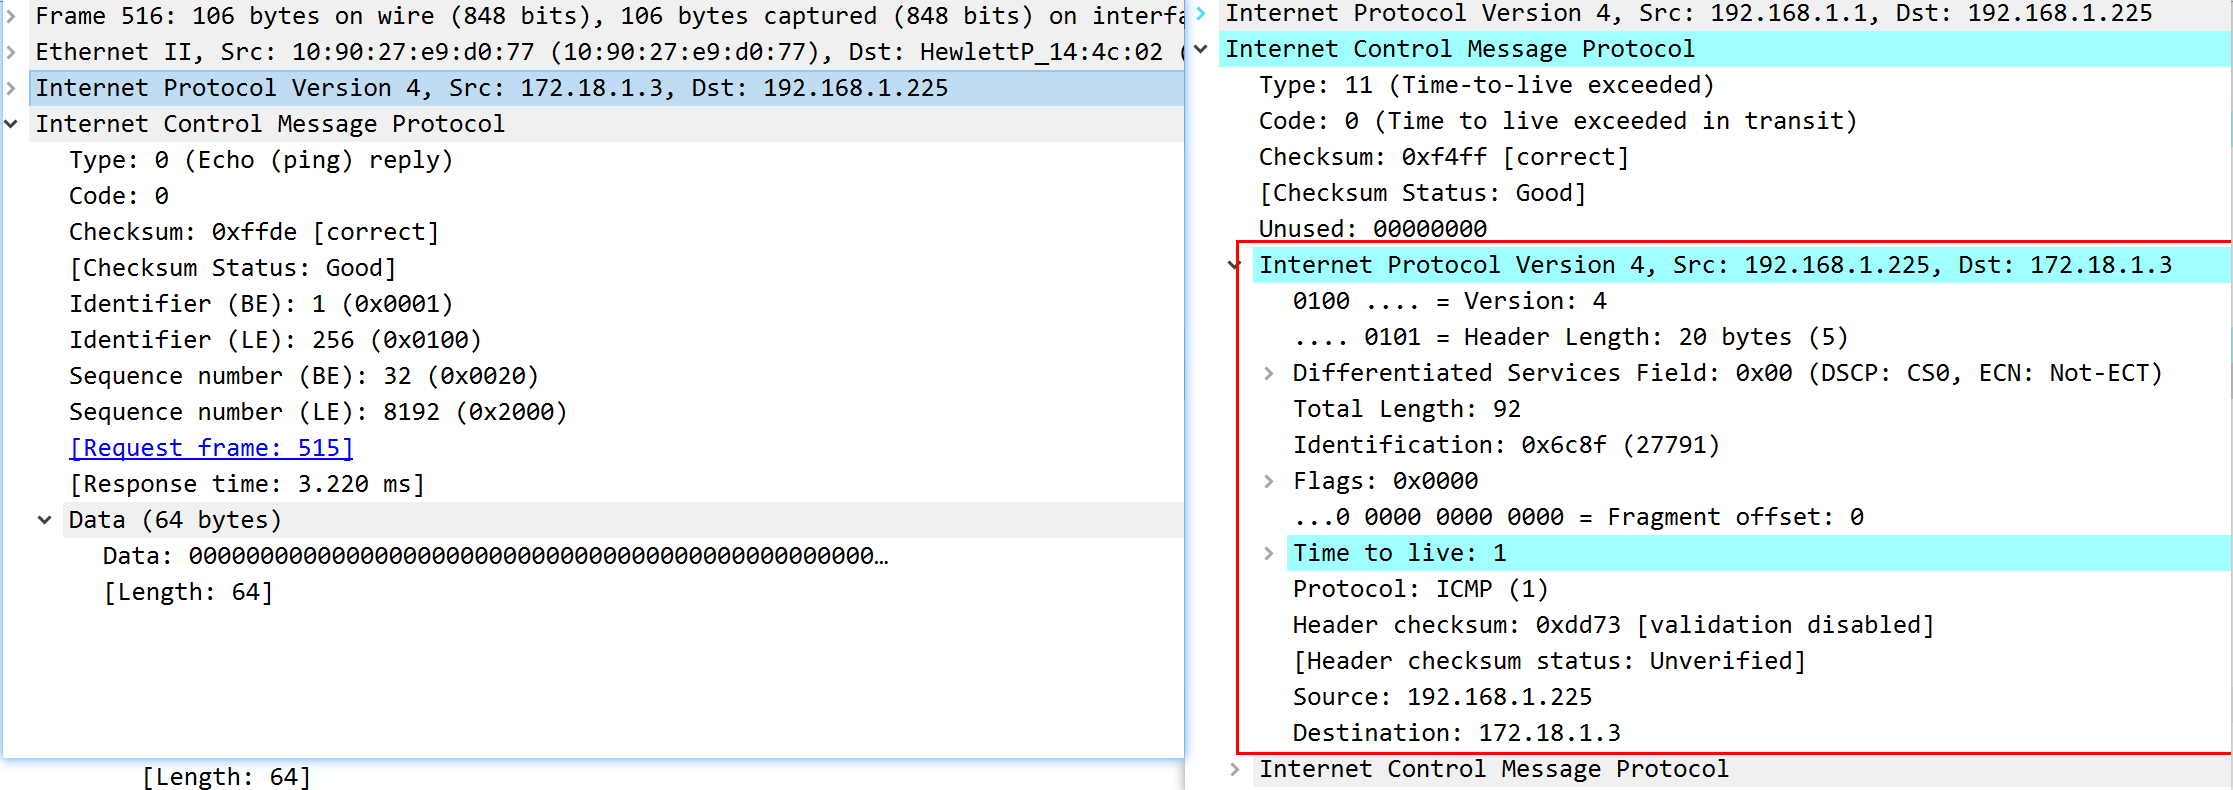
\includegraphics[width=0.8\linewidth]{assets/diff2.png}
      \caption{The TTL-exceeded packet(right) has a IPv4 datagram in it, the normal(left) has not}
    \end{figure}
    \item The TTL-exceeded packet has no data filed at second level.
    \begin{figure}[H]
      \centering
      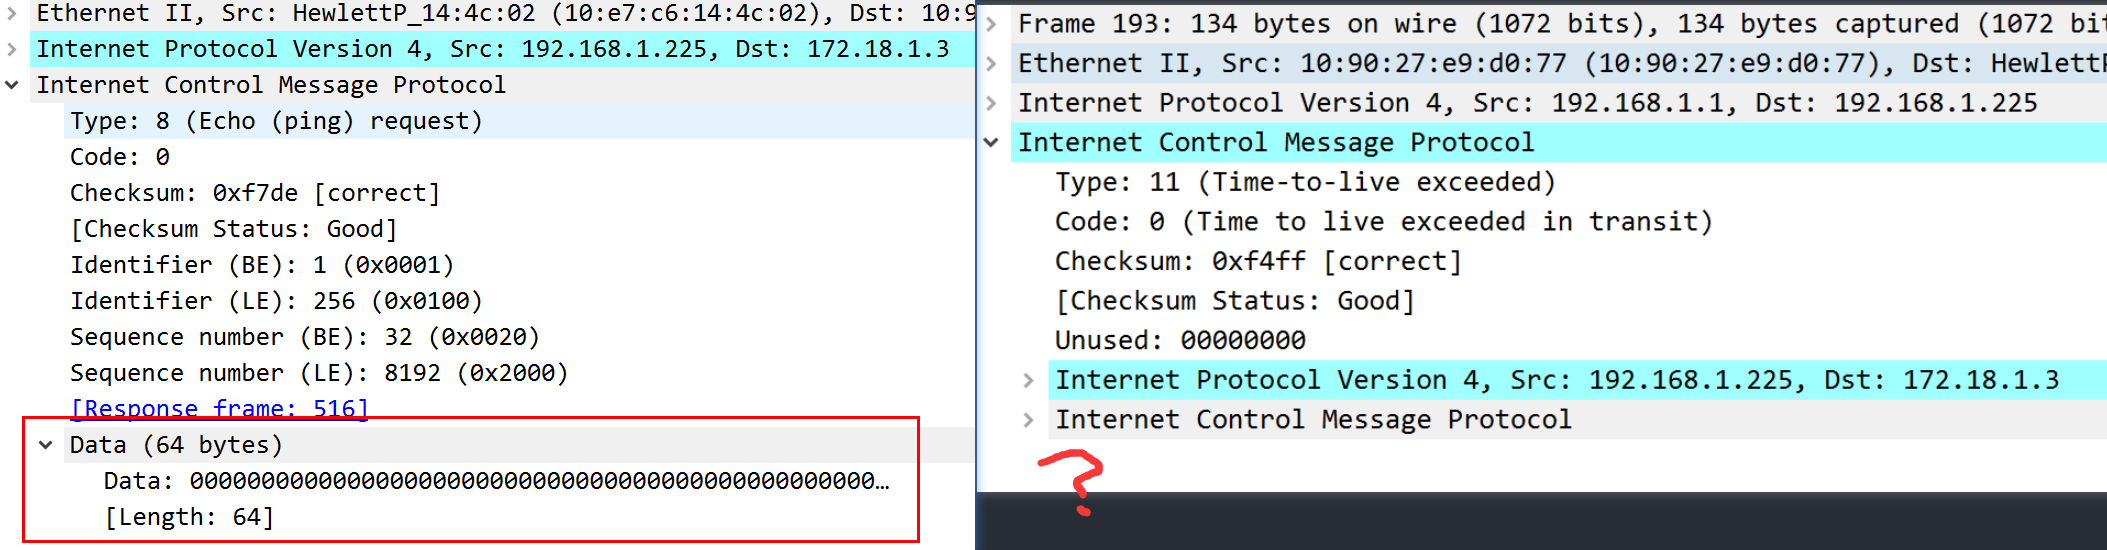
\includegraphics[width=0.8\linewidth]{assets/diff3.png}
      \caption{The TTL-exceeded packet(right) has no data at second level, the normal(left) has}
    \end{figure}
  \end{enumerate}
\end{enumerate}


\newpage


\section*{Problem 3}

{\bf Description}

Initiates a DHCP session

\begin{enumerate}
  \item How to initiate a DHCP session? How to find the DHCP session packets?
  \item What ‘s the source IP address and destination IP address of a DHCP request? What is the type of these two IP address?
  \item What info items are required for a host if it need to contact with others in the Internet?
  \item How do you find the Lease Time of a dynamic IP address? What’s the value of it? In which type of DHCP packet could this field be set?
\end{enumerate}

Please add the necessary screenshots when answering questions


{\bf Solution}

\begin{enumerate}
  \item Use \verb|ipconfig /renew| command. Use \verb|dhcp| filter in wireshark.
  \begin{figure}[H]
    \centering
    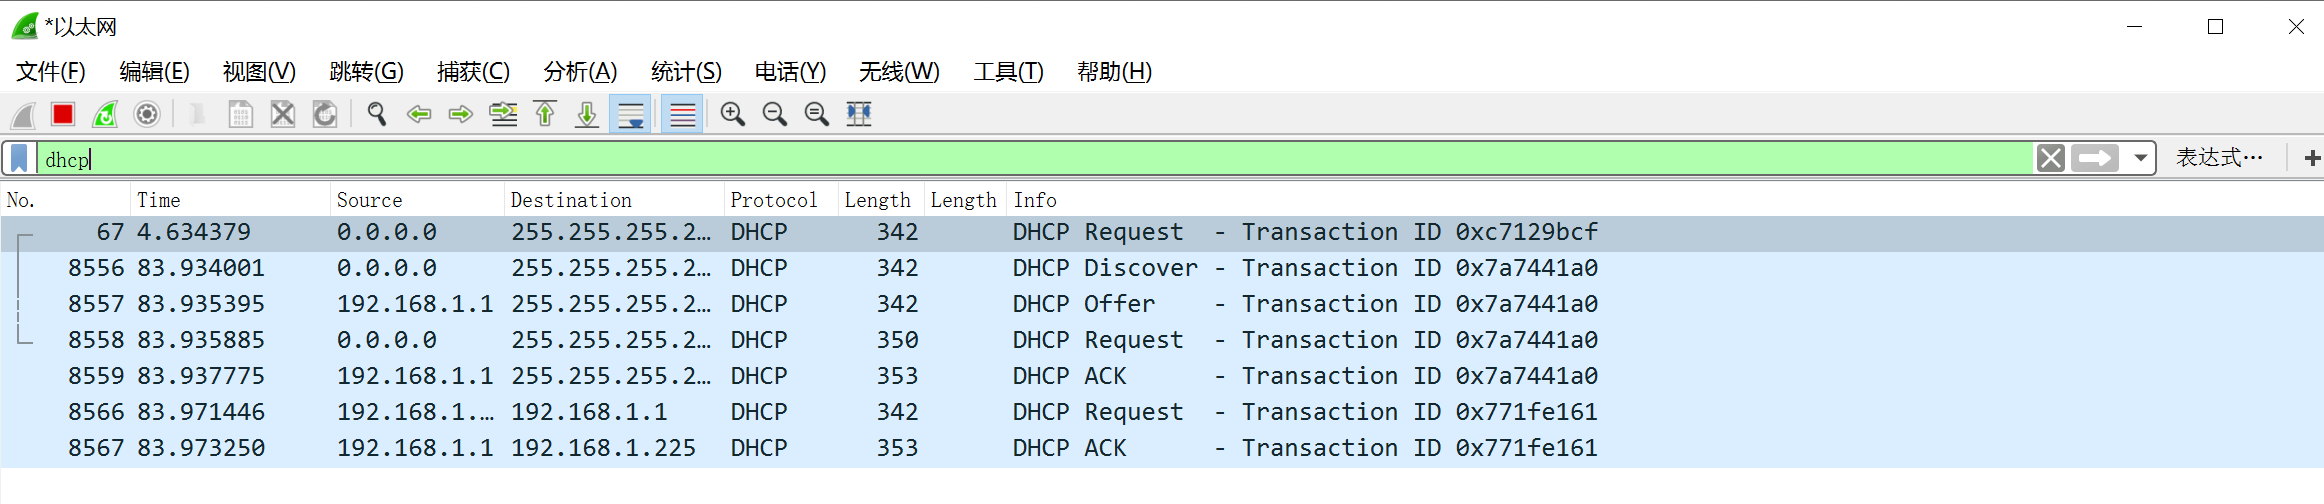
\includegraphics[width=0.8\linewidth]{assets/dhcp.png}
    \caption{DHCP session}
  \end{figure}
  \item Source IP address of a DHCP request is 0.0.0.0. Destination IP address of a DHCP request is 255.255.255.255.
  The source IP address is non-routable meta-address. The destination IP address is broadcast address.
  \item 1. IP address 2. Subnet Mask 3. Default Gateway
  \item Use \verb|ipconfig /all| command. The lease time is about 19 hours, 2 minutes and 50 seconds. The "IP Address Lease Time" filed in the DHCP packet.
  \begin{figure}[H]
    \centering
    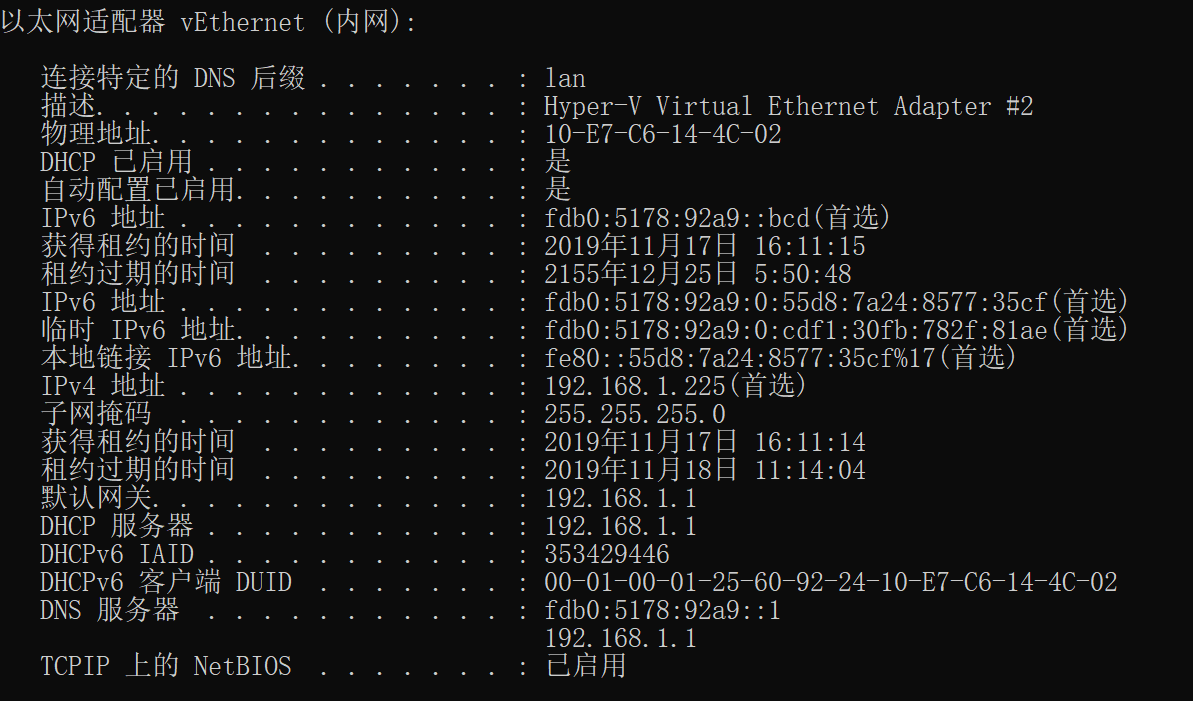
\includegraphics[width=0.8\linewidth]{assets/ipconfig.png}
    \caption{IP Lease Time}
  \end{figure}
\end{enumerate}

\end{document}
